\usetikzlibrary{calc}
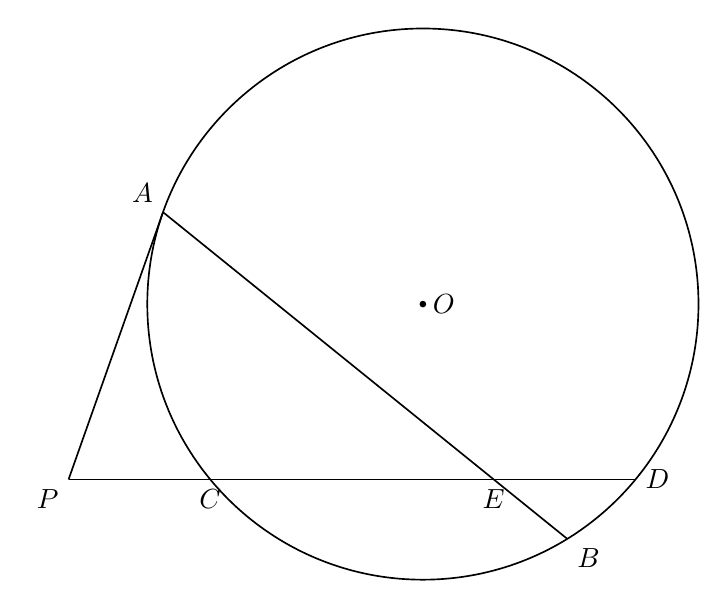
\begin{tikzpicture}[x=1cm,y=1cm,line width=.6pt,font=\normalsize]
\coordinate (P) at (0,0);
\coordinate (C) at (1.8,0);
\coordinate (E) at (5.4,0);
\coordinate (D) at (7.2,0);
\coordinate (A) at (1.2,3.394);
\coordinate (B) at (6.333,-0.754);
\coordinate (O) at (4.5,2.227);
\draw[black] (O) circle[radius=3.5cm];
\draw[black] (P)--(A);
\draw[black] (P)--(D);
\draw[black] (A)--(B);
\fill[black] (O) circle (1.2pt);
\node[below left] at (P) {$P$};
\node[below] at (C) {$C$};
\node[below] at (E) {$E$};
\node[right] at (D) {$D$};
\node[above left] at (A) {$A$};
\node[below right] at (B) {$B$};
\node[right] at (O) {$O$};
\end{tikzpicture}
